%====== BASIC PREAMBLE STUFF =======
\documentclass[11pt]{article}
\usepackage[nottoc,numbib]{tocbibind}
\usepackage{geometry} 
 \geometry{
 a4paper,
 total={170mm,257mm},
 left=1in,
 top=1in,
 bottom = 1in,
 right = 1in
 }
\usepackage{amsmath, amssymb, amsthm, lastpage, upgreek, fancyhdr, seqsplit, bm, mathrsfs, accents, transparent, dsfont, float, esint, tikz, lipsum, lmodern, hyperref, cleveref, bigints, tikz-among-us, graphicx, xcolor}
\usepackage{minted}
\usepackage[most]{tcolorbox}
\usepackage[framemethod=TikZ]{mdframed}
\hypersetup{pdfborder=0 0 0}
\usepgflibrary{arrows}
\usepackage[nodisplayskipstretch, doublespacing]{setspace}\onehalfspacing
\tcbuselibrary{theorems}
\allowdisplaybreaks

\setlength{\parindent}{0pt}


%====== ENVIRONMENTS STUFF ======
\newenvironment{solution}
{
  \begin{proof}[Solution]}
  {\end{proof}}
  
\renewcommand\qedsymbol{$\blacksquare$}

\theoremstyle{definition}
\newtheorem*{definition}{Definition}
\newtheorem*{theorem}{Theorem}
\newtheorem*{claim}{Claim}
\newtheorem*{lemma}{Lemma}
\newtheorem*{corollary}{Corollary}
\newtheorem*{proposition}{Proposition}

\newcounter{question}[section]\setcounter{question}{0}

\newenvironment{question}[2][]{%
\refstepcounter{question}%
\ifstrempty{#1}%
{\mdfsetup{%
frametitle={%
\tikz[baseline=(current bounding box.east),outer sep=0pt]
\node[anchor=east,rectangle,fill=cyan!50!
{\strut Problem};}}
}%
{\mdfsetup{%
frametitle={%
\tikz[baseline=(current bounding box.east),outer sep=0pt]
\node[anchor=east,rectangle,fill=green!20!]
{\strut Problem~#1};}}%
}%
\mdfsetup{innertopmargin=10pt,linecolor=cyan!20,%
linewidth=2pt,topline=true,%
frametitleaboveskip=\dimexpr-\ht\strutbox\relax
}
\begin{mdframed}[]\relax%
\label{#2}}{\end{mdframed}}


%====== NEW COMMANDS ======
\newcommand{\Var}{\text{Var}}
\renewcommand{\lambda}{\uplambda}
\renewcommand{\phi}{\varphi}
\newcommand{\indep}{\perp \!\!\! \perp}
\renewcommand{\epsilon}{\varepsilon}
\newcommand{\Cov}{\text{Cov}}
\newcommand{\ds}{\displaystyle}
\newcommand{\Sd}{\text{SD}}
\newcommand{\Corr}{\text{Corr}}
\newcommand{\mkt}{\text{mkt}}


%====== HEADER AND TITLE =======
\pagestyle{fancy}
\fancyhf{}
\rhead{Ian Zhang}
\lhead{ECO358 Notes}
\cfoot{Page \thepage}

\title{ECO358 Notes}
\author{Ian Zhang}

\begin{document}
\maketitle

\tableofcontents

\newpage

\section{Tools and Framework}
\subsection{Valuation Principle}
The valuation principle states that 
\begin{itemize}
    \item Value is determined by competitive market price
    \item Benefits/costs should be evaluated at market price
    \item Benefits exceeding costs equate to investing increasing market value of the firm
\end{itemize}

\subsubsection{Price of Time and Present value}

\begin{definition}
    The interest rate is the exchange rate across time. We assume a risk-free interest rate denoted $r_f$. 
\end{definition}

\begin{definition}[Simple investment]
    An investment that only earns interest on principal interest and none on accrued interest.
    \begin{equation*}
        I = I_0(1 + rt)
    \end{equation*}
    where $I_0$ is initial investment and $I$ is the value at time $t$
\end{definition}

\begin{definition}[Compounded investment]
    An investment that earns interest from both principal and accrued interest.
    \begin{equation*}
        I = I_0(1 + r)^t
    \end{equation*}
\end{definition}

\textbf{Present value formula:}
\begin{equation*}
    PV = \sum_{t=0}^n \frac{c_t}{(1 + r_f)^t} = c_0 + \frac{c_1}{1 + r_f} + \frac{c_2}{(1 + r_f)^2} + \cdots + \frac{c_n}{(1 + r_f)^n}
\end{equation*}
Present value represents \textit{today's} value of an investment opportunity.
\vspace{0.5cm}

\textbf{Future value at time $n$ formula:}
\begin{equation*}
    FV_n = \sum_{t = 0}^n c_t(1 + r_f)^t = c_0 + c_1(1 + r_f) + c_2(1 + r_f)^2 + \cdots + c_n(1 + r_f)^n
\end{equation*}

\begin{definition}[Net Present Value]
    The difference between present value of an investment's benefits and costs
    \begin{equation*}
        NPV = PV(\text{benefits})  - PV(\text{costs})
    \end{equation*}
\end{definition}
\begin{itemize}
    \item If $NPV < 0$, we choose to not invest since the price of the investment would be higher than the present value of the benefits (i.e.: the investment is too costly)
    \item If presented with multiple investment opportunities, we choose the one with the highest $NPV$ as it would be equivalent to receiving the $NPV$ today (this opportunity has the best cost-benefit ratio)
    \item $PV(\text{costs})$ is just the price of the investment opportunity today (i.e.: price of the stock)
\end{itemize}

\begin{definition}[Internal Rate of Return]
    The interest rate at which $NPV = 0$.
\end{definition}

\subsection{Law of One Price}
\subsubsection{Arbitrage}
\begin{definition}[Arbitrage]
    The buying and selling of similar goods in different markets to take advantage of price differences
\end{definition}
\begin{definition}[Normal market]
    A market without any arbitrary opportunities.
\end{definition}
\subsubsection{No-Arbitrage Price of Security}
Unless 
\begin{equation*}
    \text{Price}(\text{Security}) = PV(\text{Cash flows from security})
\end{equation*}
an arbitrage opportunity will appear.
\begin{itemize}
    \item In a normal market, $NPV$ of buying/selling a security is $0$ since there is no arbitrage
\end{itemize}

\subsection{Perpetuities and Annuities}
\subsubsection{Perpetuity}
\begin{definition}[Perpetuity]
    A constant cash flow that occurs at regular intervals \textbf{forever}
    \begin{equation*}
        PV_{\text{perpetuity}} = PV_0 = \frac{c}{r}
    \end{equation*}
    where $c$ is the constant cash flow and $r$ the rate of return
\end{definition}
\begin{proof}
    By the formula for present value,
    \begin{align*}
        PV_0 &= \sum_{t=1}^\infty \frac{c}{(1 + r)^t}\\
        (1 + r)PV_0 &= \sum_{t =1}^\infty \frac{c}{(1 + r)^{t - 1}}\\
        (1 + r)PV_0 - PV_0 &= c\\
        PV_0 &= \frac{c}{r}
    \end{align*}
\end{proof}
Notice how $t$ starts at $1$ since we receive the first $c$ payment at the end of the first interval. An equivalent type of question asked will be about how much money to put in right now to finance a perpetuity of cash flow $c$ at a rate of $r$. If the first payment is today as opposed to at the end of the first period, then 
\begin{equation*}
    PV_0 = \frac{c}{r} + c
\end{equation*}

\subsubsection{Annuity}
\begin{definition}[Annuity]
    A constant cash flow that occurs at regular intervals for a \textbf{finite} number of $n$ periods
    \begin{equation*}
        PV_{\text{annuity}} = \frac{c}{r} - \frac{c}{r}\frac{1}{(1 + r)^n}
    \end{equation*}
    where $c$ is the constant cash flow and $r$ the rate of return
\end{definition}
\begin{proof}
    By formula for present value,
    \begin{align*}
        PV_0 &= \sum_{t=1}^n \frac{c}{(1 + r)^t}\\
        (1  +r)PV_0 &= \sum_{t=1}^n \frac{c}{(1 + r)^{t-1}}\\
        (1 + r)PV_0 - PV_0 &= c - \frac{c}{(1 + r)^n}\\
        PV_0 &= \frac{c}{r} - \frac{c}{r}\frac{1}{(1 + r)^n}
    \end{align*}
\end{proof}
Similarly, if the first payment is today as opposed to at the end of the first interval, 
\begin{equation*}
    PV_0 = \frac{c}{r} - \frac{c}{r}\frac{1}{(1 + r)^n} + c
\end{equation*}
\subsubsection{Growing Cash Flows}
Assuming the cash flow grows at a constant rate of $g$ (i.e. The cash flow at the end of period 2 is $c(1 + g)$), 
\begin{equation*}
    PV_{\text{perpetuity}} = \frac{c_1}{r - g} \qquad PV_{\text{annuity}} = \frac{c_1}{r-g} - \frac{c_1}{r-g}\left(\frac{1+g}{1 + r}\right)^n
\end{equation*}

\subsection{Interest Rates}
\subsubsection{Effective Annual Rate}
\begin{definition}[Effective Annual Rate (EAR)]
    The total amount of interest that will be earned at the end of one year
    \begin{itemize}
        \item \textbf{Considers} compounding
    \end{itemize}
    \begin{equation*}
        EAR = (1 + r)^k - 1
    \end{equation*}
    where $k$ is the number of compounding periods per year, $r$ is the effective interest rate per compounding period
\end{definition}

\subsubsection{Annual Percentage Rate}
\begin{definition}[Annual Percentage Rate (APR)]
    The amount of interest earned in one year \textbf{without considering} compounding
    \begin{equation*}
        r = \frac{APR}{k \text{ periods/year}}
    \end{equation*}
\end{definition}
Note that by definition,
\begin{equation*}
    APR \leq EAR
\end{equation*}
where equality happens only for annual compounding.

\subsubsection{Converting APR to EAR}
Given 
\begin{equation*}
    EAR = (1 + r)^k - 1
\end{equation*}
and 
\begin{equation*}
    APR = \frac{APR}{k}
\end{equation*}
then 
\begin{equation*}
    EAR = \left(1 + \frac{APR}{k}\right)^k - 1
\end{equation*}

\subsubsection{Inflation and Real/Nominal Rates}
\begin{definition}[Nominal interest rate]
    The interest rate quoted by financial institutions.
\end{definition}
\begin{definition}[Real interest rate]
    The interest rate adjusted for inflation.
\end{definition}
Let $r_r$ be real interest rate, $r$ be nominal rate, $i$ be inflation rate. Then
\begin{equation*}
    r_r = \frac{r-i}{1 + i}
\end{equation*}

\section{Bonds}
\subsection{Bond Valuation and Bond Prices}
\begin{definition}[Bond certificate]
    States the terms of the bond.
\end{definition}
\begin{definition}[Maturity date]
    The final repayment date of the bond
\end{definition}
\begin{definition}[Term]
    The time remaining until repayment is due (time until maturity).    
\end{definition}
\begin{definition}[Coupon]
    A promised interest payment that comes with the bond contract.
\end{definition}
\begin{definition}[Face value]
    The promised repayment amount made out to the buyer by the seller at maturity.
\end{definition}
\begin{definition}[Coupon rate]
    The rate that determines the amount of each coupon payment (similar to what $APR$ is).
\end{definition}

\begin{equation*}
    CPN = \frac{\text{Coupon rate} \times \text{Face value}}{\text{No. coupon payments per year}}
\end{equation*}

\subsubsection{Zero-coupon Bonds}
First, assume there are no coupon payments. 
\begin{definition}[Treasury bills]
    Government of Canada bonds that are zero-coupon bonds with a maturity of up to a year.
\end{definition}

\begin{definition}[Yield to maturity]
    The discount rate that sets $PV$ of the promised bond equal to the current market price of the bond ($YTM$ is the $IRR$ of a bond)
    \begin{itemize}
        \item Sets $NPV = 0$
    \end{itemize}
    \begin{equation*}
        YTM = \left(\frac{FV}{P}\right)^{\frac{1}{n}} - 1
    \end{equation*}
    where $FV$ is the face value, $P$ the price, $n$ the length of the contract.
\end{definition}

\subsubsection{Spot Rate of Interest}
\begin{definition}[$n$-period rate of interest]
    The rate appropriate for discounting a risk-free cash flow that occurs on date $n$, denoted $r_n$
\end{definition}
\begin{itemize}
    \item A default-free zero-coupon bond that matures on date $n$ provides a risk-free return over the same period at interest rate $r_n$
    \begin{itemize}
        \item[$\circ$] The Law of One Price guarantees that 
        \begin{equation*}
            r_n  = YTM_n
        \end{equation*}
        or else an arbitrage opportunity exists
    \end{itemize}
\end{itemize}

\subsubsection{Coupon Bonds}
A coupon bond pays both a face value at maturity and regular coupon interest payments throughout the duration of the contract.
\begin{equation*}
    P = \frac{CPN}{YTM}\left(1 - \frac{1}{(1 + YTM)^n}\right) + \frac{FV}{(1 + YTM)^n}
\end{equation*}
\begin{itemize}
    \item Treat the coupon payments like an annuity 
\end{itemize}

\subsubsection{Dynamic Behaviour of Bond Prices}
\begin{definition}
    A bond is selling at a \textbf{discount} if $P < FV$
    \begin{itemize}
        \item Coupon rate is less than $YTM$
    \end{itemize}
\end{definition}
\begin{definition}
    A bond is selling at \textbf{par} if $P = FV$
\end{definition}
\begin{definition}
    A bond is selling at a \textbf{premium} if $P > FV$
    \begin{itemize}
        \item Coupon rate is greater than $YTM$
    \end{itemize}
\end{definition}
Note that a bond's yield of maturity will \textbf{not} change over time and the price of a discount/premium bond will move towards par value over time 
\begin{itemize}
    \item Regardless of the coupon rate, the bond value will gradually converge to $FV$ closer to the maturity date
\end{itemize}
This means that even if we sell the bond early, the $IRR = YTM$ regardless, which preserves a normal market (i.e.: no arbitrage opportunity is presented).

\subsubsection{Interest Rates and Bond Prices}
\begin{itemize}
    \item Interest rate changes are inversely related with bond prices.
    \begin{itemize}
        \item The higher the bond's duration, the higher the sensitivity to interest rate changes
    \end{itemize}
\end{itemize}

\subsection{Yield Curves and Bond Arbitrage}
Given a coupon bond, its possible to decompose it into a series of zero-coupon bonds
\begin{itemize}
    \item Can determine the price and yield of default free bonds by considering the Law of One Price and yields of default-free zero coupon bonds
    \item Keep in mind that the price of a bond must be equal to the present value of the bond's coupon payments and face value, or else an arbitrage opportunity is presented
    \begin{equation*}
        P = PV = \sum_{t = 1}^n \frac{CPN}{(1 + r_t)^t} + \frac{FV}{(1 + r_n)^n}
    \end{equation*}
\end{itemize}

\subsection{Corporate Bonds}
\begin{definition}[Corporate bonds]
    Bonds that are issue by corporations.  
\end{definition}
\begin{definition}[Credit risk]
    The risk of default.
\end{definition}
An investor is willing to pay less for bonds with credit risk than identical default-free bonds, thus the yield of credit risk bonds is greater than otherwise identical default-free bonds. 
\begin{definition}[Credit spread]
    The difference between yields of corporate bonds and treasury yields
\end{definition}
Consider a zero-coupon bond with uncertain bond payoffs with a face value of 1000. Assume
\begin{enumerate}
    \item 50\% chance of repaying its face value
    \item 50\% chance of default and receiving 90\% of the face value
\end{enumerate}
The expected amount to receive is calculated using expectation:
\begin{equation*}
    .5(1000) + .5(900) = 950
\end{equation*}
\begin{itemize}
    \item Bonds with a risk of default will have a discount rate $d$ that serves as the interest rate used to calculate the present value of the bond
\end{itemize}

\subsection{Forward Interest Rates}
\begin{definition}[Forward Interest Rates]
    The interest rate that we can guarantee today for a loan/investment that will occur in the \textbf{\textit{future}}
\end{definition}
\begin{itemize}
    \item The forward rate for year $n$, $f_n$, is the rate available today on a one-year investment that begins $n-1$ years from today
    \begin{itemize}
        \item The forward rate for year $1$ is equivalent to an investment on a one-year zero-coupon bond
        \begin{equation*}
            f_1 = r_1
        \end{equation*}
    \end{itemize}
\end{itemize}
In general, by the Law of One Price,
\begin{equation*}
    (1 + r_n)^n = (1 + r_{n-1})^{n-1}(1 + f_n)
\end{equation*}
Thus
\begin{equation*}
    f_n = \frac{(1 + r_n)^n}{(1 + r_{n-1})^{n-1}} - 1
\end{equation*}
This implies that the bond yields of zero-coupon bonds is given by
\begin{equation*}
    (1 + r_n)^n = \prod_{k=1}^n (1 + f_k)
\end{equation*}
\begin{itemize}
    \item The $r_n$ are also known as \textit{short rates}
\end{itemize}

\subsubsection{Uncertainty in Interest Rates and Forward Rates}
Suppose we have today's rate $r_1$ and expected short rate of year $2$, $E(r_2)$. If we want to invest for 1 year, we could:
\begin{enumerate}
    \item Buy a 2 year bond and plan to sell it after a year for a price of 
    \begin{equation*}
        \frac{FV}{1 + E(r_2)}
    \end{equation*}
    \item Buy a 1 year bond and hold to maturity
\end{enumerate}
The issue with the first option is that we don't actually know how much we can sell the bond for after a year; it's based on an \textit{expected} short rate.\\
Generally, a risk premium is required for longer-term bonds, called a \textit{liquidity premium}. This liquidity premium compensates short-term investors for uncertainty about future prices
\begin{equation*}
    f_n = E(r_n)  + \text{liquidity premium}
\end{equation*}

\subsubsection{Term Structure and Yield Curves}
\begin{definition}[Term structure]
    The relationship between investment term and interest rate. This is graphed by the yield curve. 
\end{definition}
The yield curve reflects expectations of future interest rates, which are clouded by liquidity premiums.
\begin{itemize}
    \item Upward sloping yield curve indicates an expectation for a rise in rates and a requirement for large liquidity premiums to hold long term bonds
\end{itemize}

\subsubsection{Term Structure Theories}
\textbf{\underline{Expectations Hypothesis Theory}}
\begin{itemize}
    \item Observed long term rate is a function of today's and expected future short term rates.
    \item Liquidity premiums are $0$ and $f_n = E(r_n)$
\end{itemize}
\textbf{\underline{Liquidity Preference Theory}}
\begin{itemize}
    \item Long term bonds are more risky, so $f_n > E(r_n)$
    \item Require a liquidity premium, which is $f_n - E(r_n)$
\end{itemize}

\section{Valuing Stocks}
\begin{definition}[Equity]
    An ownership share in a firm
\end{definition}

\subsection{Dividend Discount Model}
With stocks, potential cash flows come from dividends and selling of the stock. 
\begin{itemize}
    \item Cash flows are risky, so we must discount them at the equity cost of capital, $r_E$
    \item Dividends can fluctuate, as opposed to the fixed coupon payments of bonds
\end{itemize}
Consider a one year investment: in 1 year, the investor gets a dividend payment of $Div_1$ and sells the stock for $P_1$, thus today's price of the stock is
\begin{equation*}
    P_0 = \frac{Div_1 + P_1}{1 + r_E}
\end{equation*}
This value is representative of the present value of the stock today
\begin{itemize}
    \item If the market price of the stock is higher than this, then investors will rush to \textit{sell} the stock, which drives the market price down
    \item If the market price of the stock is lower than this, then investors will rush to \textit{buy} the stock, which drives the market price up
\end{itemize}
Notice we can rearrange the above equation to 
\begin{equation*}
    r_E = \frac{Div_1 + P_1}{P_0} - 1 = \underbrace{\frac{D i v_1}{P_0}}_{\text {Dividend Yield }}+\underbrace{\frac{P_1-P_0}{P_0}}_{\text {Capital Gain Rate }}
\end{equation*}

\subsubsection{Multi-Year Investing}
For $N$ years,
\begin{equation*}
    P_0 = \sum_{k=1}^N \frac{Div_k}{(1 + r_E)^k} + \frac{P_N}{(1 + r_E)^N}
\end{equation*}
Suppose $N \to \infty$.\\
\textbf{\underline{Dividend Discount Model:}}\\
The value of a firm is an infinite stream of discounted dividend payments
\begin{equation*}
    P_0 = \sum_{k=1}^\infty \frac{Div_k}{(1  + r_E)^k}
\end{equation*}
\textbf{Constant Dividend Growth:} The simple forecast for a firm's future dividends is that they grow at a constant rate $(g)$ forever, so $Div_n = Div_1(1 + g)^{n-1}$
\begin{equation*}
    P_0 = \frac{Div_1}{r_E - g} \iff r_E = \frac{Div_1}{P_0} + g
\end{equation*}
Note the above equations follow from the formula for an infinite geometric sum:
\begin{equation*}
    \sum_{k=0}^\infty ar^k = \frac{a}{1-r} = \sum_{k=1}^\infty ar^{k-1}
\end{equation*}
\subsubsection{Simple Model of Growth}
\begin{definition}[Dividend Payout Ratio]
    The fraction of earnings paid as dividends each year
    \begin{equation*}
        Div_t  = \underbrace{\frac{\text{Earnings}_t}{\text{Shares outstanding}_t}}_{EPS_t} \times \text{Dividend Payout Rate}_t
    \end{equation*}
\end{definition}
\begin{equation*}
    \text{Change in Earnings} = \text{New Investment} \times \text{Return on New Investment}
\end{equation*}
where 
\begin{equation*}
    \text{New Investment} = \text{Earnings} \times \text{Retention Rate}
\end{equation*}
where retention rate is the fraction of current earnings that the firm retains each year. 
\begin{equation*}
    \text{Earnings Growth Rate} = \frac{\text{Change in Earnings}}{\text{Earnings}} = \text{Retention Rate} \times \text{Return on New Investment}
\end{equation*}
If a firm chooses to keep its dividend payout rate constant, then
\begin{equation*}
    g = \text{Retention Rate} \times \text{Return on New Investment}
\end{equation*}
or in other words, the dividend growth rate is equal to the earnings growth rate.
\subsection{Valuation Based on Comparable Firms}
Note that both the growth rate of earnings and growth rate of dividends are denoted the same but are different because if there is repurchasing of shares, then the growth rate of dividends is higher than the growth rate of earnings due to a portion of the retained capital going into the repurchasing of shares.
\begin{equation*}
    P/ E\text{ ratio} = \frac{P}{EPS} = \frac{Div_1}{r_E-g}\frac{1}{EPS} = \frac{\text{Dividend Payout Ratio}}{r_E - g}
\end{equation*}
The $P/E$ ratio estimates the value of a firm based on the value of another comparable firm that we expect will generated similar cash flows in the future.

\section{Risk and Return}
With risk, there are different returns that may be yielded with different likelihoods
\subsection{Expected Returns}
\begin{equation*}
    E(R) = \sum_R P_R R
\end{equation*}

\subsection{Variance and Standard Deviation}
\begin{equation*}
    \Var(R) = E[(R - E(R))^2] = \sum_R P_R (R - E(R))^2
\end{equation*}
\begin{equation*}
    \Sd(R) = \sqrt{\Var (R)}
\end{equation*}

\subsection{Historical Returns and Tradeoff}
\begin{definition}[Realized Return]
    The return that actually occurs in a time period
    \begin{equation*}
        R_{t +1 } = \frac{Div_{t + 1} + P_{t + 1}}{P_t} -1
    \end{equation*}
\end{definition}
\begin{definition}[Realized Annual Returns]
    If a stock pays dividends at the end of each quarter with realized returns 
    \begin{equation*}
        R_{Q_1}, R_{Q_2}, R_{Q_3}, R_{Q_4}
    \end{equation*}
    then its realized annual return is 
    \begin{equation*}
        1 + R_{\text{annual}} = (1 + R_{Q_1}) (1 + R_{Q_2}) (1 + R_{Q_3}) (1 + R_{Q_4})
    \end{equation*}
\end{definition}

\subsubsection{Average Annual Return}
\begin{equation*}
    \bar R  = \frac{1}{T}\sum_{i=1}^T R_i  
\end{equation*}

\subsubsection{Variance and Volatility of Returns}
\begin{align*}
    \Var(R) &= \frac{1}{T-1} \sum_{i=1}^T (R_i - \bar R)^2\\
    \Sd(R) &= \sqrt{\Var(R)}
\end{align*}
Problems with using past returns to predict the future expected returns:
\begin{enumerate}
    \item Don't know what investors expected in the past; can only observe actual realized returns
    \item $\bar R$ is an estimator $E(R)$
    \begin{itemize}
        \item Individual stocks tend to be more volatile than large portfolios
        \item Average returns earned in the past are not reliable estimators for future expected returns
    \end{itemize}
\end{enumerate}

\subsubsection{Estimation Error}
\begin{definition}[Standard Error]
    A statistical measure of the degree of estimation error
    \begin{itemize}
        \item Standard error of $\bar R$ is 
        \begin{equation*}
            \Sd(\bar R) = \frac{\Sd(\text{Independent Risk})}{\sqrt{\text{Number of observations}}} = \frac{\Sd(R_1)}{\sqrt{n}}
        \end{equation*}
        \item $95\%$ confidence interval is 
        \begin{equation*}
            \bar R \pm 2 \times \Sd(\bar R)
        \end{equation*}
    \end{itemize}
\end{definition}
\begin{definition}[Excess Returns]
    Difference between average return for an investment and average return of T-Bills.
\end{definition}

\subsection{Diversification of Risk}
There are 2 types of risk:
\begin{enumerate}
    \item Common risk: perfectly correlated risk
    \begin{itemize}
        \item Affects all securities; also known as systematic risk
    \end{itemize}
    \item Independent risk: uncorrelated risk
    \begin{itemize}
        \item Affects a particular security
        \item Can be diversified
    \end{itemize}
\end{enumerate}
\begin{definition}[Diversification]
    Averaging out of independent risks in a large portfolio.
\end{definition}

\subsubsection{Diversification in Stock Portfolios}
\begin{itemize}
    \item Holding a portfolio of only Type S firms (firms that face the same systematic risk) will not diversify the risk, since if one firm flops then all others do too. Investing in a portfolio of Type S firms is effectively investing in 1 firm. 
    \item Holding a portfolio of only Type I firms (firms that face firm-specific risk) will diversify the risk, since if one flops, the others may not
\end{itemize}

The risk premium for diversifiable risk is 0 since if otherwise, an investor could buy a portfolio and earn the risk premiums whilst diversifying away the risk. Therefore, the risk premium is determined by \textbf{systematic risk}.

\subsection{Market Beta}
\begin{definition}[Beta ($\beta$)]
    The expected percent change in the excess return of a security for a 1$\%$ change in the excess return of the market portfolio
\end{definition}
\begin{itemize}
    \item $\beta$ only measures systematic risk, not total risk
    \begin{itemize}
        \item Since $\beta$ measures only systematic risk, the $\beta$ of a firm gives a metric on the amount of un-diversifiable risk the security carries
    \end{itemize}
    \item $\beta \neq \Sd(R)$
    \item Since a Type I form faces no systematic risk, its beta is $0$. This makes sense since the returns of a Type I firm's stock are not dependent on market conditions
    \item In other words, $\beta$ is a measure of a security's sensitivity to market-wide risk factors
\end{itemize}

\begin{definition}[Market Risk Premium]
    The reward investors expect to earn for holding a portfolio with a beta of $1$ (aka the market portfolio)
    \begin{itemize}
        \item How much an investor needs to be compensated for investing in the market portfolio
    \end{itemize}
    \begin{equation*}
        \text{Market Risk Premium} = E[R_{mkt}] - r_f
    \end{equation*}
\end{definition}
Since $\beta_i$ measures the sensitivity of firm $i$ to market risk factors, then the risk premium of firm $i$ is 
\begin{equation*}
    \beta_i\times \text{Market Risk Premium}
\end{equation*}
\begin{equation}\label{capm}
    E(R_i) = r_f + \beta_i(E(R_{mkt}) - r_f)
\end{equation}
Equation (\ref{capm}) is known as the \textbf{Capital Asset Pricing Model, or CAPM}, where $E(R_i)$ tells us the equity cost of capital for firm $i$.

\subsection{Return and Volatility of Portfolios}
\begin{definition}[Portfolio Weight]
    The fraction of the total investment in the portfolio held in each individual investment in the portfolio
    \begin{equation*}
        x_i = \frac{\text{Value of investment }i}{\text{Total value of portfolio}}
    \end{equation*}
    Note that the $x_i$ must add up to $1$.
\end{definition}
\begin{definition}[Portfolio Return ($R_p)$]
    The weighted average of the returns on the investments in the portfolio, where the weights are the corresponding portfolio weights
    \begin{equation*}
        R_p = \sum_{i=1}^n x_i R_i
    \end{equation*}
    assuming there are $n$ investments in the portfolio.
\end{definition}
\begin{itemize}
    \item The expected return of a portfolio is obtained by taking expectation of the portfolio return:
    \begin{equation*}
        E(R_p) = E\left(\sum_{i=1}^n x_iR_i\right) = \sum_{i=1}^n x_i E(R_i)
    \end{equation*}
\end{itemize}
\subsubsection{Covariance and Correlation}
\begin{definition}[Covariance]
    The expected product of the deviations of two returns from their means
    \begin{itemize}
        \item Measures how two returns move together
    \end{itemize}
    \begin{equation*}
        \Cov(R_i, R_j) = E[(R_i - E(R_i))(R_j - E(R_j))]
    \end{equation*}
\end{definition}
An estimator of covariance can by obtained by 
\begin{equation*}
    \overline{\Cov}(R_i, R_j) = \frac{1}{T-1}\sum_{t} (R_{i, t} - \bar R_i)(R_{j, t} - \bar R_j)
\end{equation*}
\begin{definition}[Correlation]
    A measure of the common risk shared by stocks that does not depend on their volatility
    \begin{equation*}
        \Corr(R_i, R_j) = \frac{\Cov(R_i, R_j)}{\Sd(R_i)\Sd(R_j)}
    \end{equation*}
\end{definition}
The variance of a portfolio is 
\begin{align*}
    \Var(R_p)  &= \Cov(R_p, R_p)\\
    &= \sum_{i=1}^n x_i \Cov(R_i, R_p)\\
    &= \sum_{i=1}^n x_i\Cov\left(R_i, \sum_{i=1}^n x_i R_i\right)\\
    &= \sum_{i=1}^n \sum_{j=1}^n x_ix_j \Cov(R_i, R_j)
\end{align*}
If the portfolio is equally weighted, then all $x_i = \frac{1}{n}$, thus 
\begin{equation*}
    \Var(R_p) = \frac{1}{n^2}\sum_{i=1}^n \Var(R_i) + \frac{1}{n^2}\sum_{i=1}^n\sum_{j=1}^n \Cov(R_i, R_j)
\end{equation*}
Define 
\begin{equation*}
    \overline{\Var}(R_p) = \frac{1}{n}\sum_{i=1}^n \Var(R_i)
\end{equation*}
\begin{equation*}
    \overline{\Cov} = \frac{1}{n(n-1)}\sum_{i=1}^n\sum_{j=1}^n \Cov(R_i, R_j)
\end{equation*}
thus we rewrite 
\begin{equation*}
    \Var(R_p) = \frac{1}{n}\overline{\Var}(R_p) + \frac{n-1}{n}\overline{\Cov}
\end{equation*}
For a portfolio with arbitrary weights,
\begin{equation*}
    \Sd(R_p) = \sum_{i=1}^n x_i \Sd(R_i)\Corr(R_i, R_p)
\end{equation*}

\subsection{Efficient Portfolios}
\begin{definition}[Efficient Portfolio]
    A portfolio such that there is no way to reduce the volatility of the portfolio without lowering its expected return
\end{definition}
\begin{definition}[Inefficient Portfolio]
    A portfolio such that there is a way to find another portfolio that is better in terms of both expected return and volatility
\end{definition}
\begin{itemize}
    \item Correlation has no effect on the expected return of a portfolio
    \item However, since correlation is dependent on volatility, it has an effect on volatility
    \item The smaller the correlation, the greater the risk reduction potential
    \begin{itemize}
        \item This is because the smaller the correlation, the easier it is to diversify away the risk
    \end{itemize}
    \begin{enumerate}
        \item If $\rho = 1$, no further risk reduction is possible since the stocks move exactly together
        \item If $\rho = -1$, then a riskless hedge is possible
    \end{enumerate}
\end{itemize}

\begin{definition}[Minimum Variance Portfolio]
    The portfolio composed of risky assets with smallest standard deviation
    \begin{itemize}
        \item The portfolio with the smallest amount of risk
    \end{itemize}
\end{definition}
Since 
\begin{equation*}
    \sigma_P^2 = x_a^2\sigma_a^2 + x_b^2\sigma_b^2 + 2x_ax_b\Cov(R_a, R_b)
\end{equation*}
then since $x_b = 1 - x_a$, we have 
\begin{equation*}
    x_{\min}(b) = \frac{\sigma_a^2 - \Cov(R_a, R_b)}{\sigma_a^2 + \sigma_b^2 - 2\Cov(R_a, R_b)}
\end{equation*}

\subsection{Short Sales}
\begin{definition}[Long position]
    A positive investment in a security
\end{definition}
\begin{definition}[Short position]
    A negative investment in a security
    \begin{itemize}
        \item Basically, a short is selling a stock that you don't own and then buying that stock back in the future
        \item Advantageous if we expect a stock price to decrease in the future
        \item Think of a short sale as investing a negative amount into a stock; it doesn't contribute to the value of the portfolio since we \textit{sold} the stock at $x$ value
    \end{itemize}
\end{definition}

\subsection{Risk-free Savings and Borrowing}
Risk can also be reduced by investing a portion of the portfolio in risk-free investments, such as T-Bills
\begin{itemize}
    \item Reduces the expected return
    \item A risk loving investor could also choose to short the risk-free investment; essentially \textit{borrow} money to invest even more into the stock market, which provides a higher expected return
\end{itemize}
If an investor chooses to invest part of his portfolio in risk-free investments, the breakdown is as follows:
\begin{enumerate}
    \item Fraction $x$ in a risky portfolio
    \item Fraction $(1 - x)$ in a risk-free investment
    \begin{itemize}
        \item If choosing to short the risk-free investment, $x$ would be greater than $1$, since the investor has more cash to invest into stocks
    \end{itemize}
\end{enumerate}
A portfolio that consists of a short position in the risk-free investment is a \textbf{levered portfolio}. The expected return of the complete portfolio is 
\begin{equation*}
    E(R_{xP}) = (1 - x)r_f + xE(R_P) = r_f + x(E(R_p) - r_f)
\end{equation*}
The standard deviation is 
\begin{equation*}
    \Sd(R_{xP}) = \sqrt{x^2 \Var(R_p)} = x\Sd(R_p)
\end{equation*}
since the volatility of the risk-free investment is $0$, and the covariance between the risky investment and the risk-free investment is $0$.
\begin{figure}[h]
    \centering
    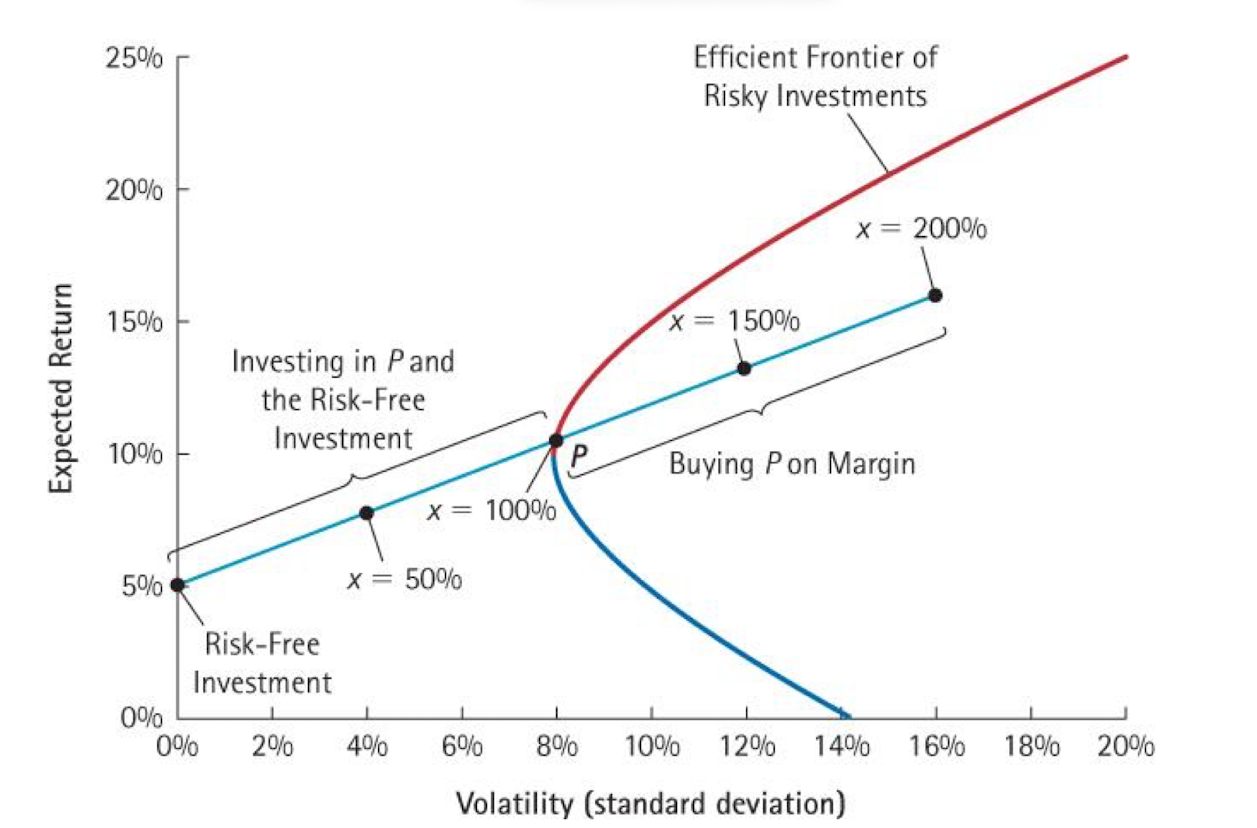
\includegraphics[scale=0.25]{Screenshot 2023-10-29 at 02.33.48.png}
\end{figure}
To earn the highest possible expected return for any level of volatility, we want to find the portfolio that generates the steepest possible line 
\begin{itemize}
    \item This line would touch the efficient frontier tangentially
\end{itemize}
\begin{definition}[Sharpe Ratio]
    The ratio of reward-to-volatility provided by a portfolio
    \begin{equation*}
        \text{Sharpe Ratio} = \frac{\text{Portfolio Excess Return}}{\text{Portfolio Volatility}} = \frac{E(R_p) - r_f}{\Sd(R_p)}
    \end{equation*}
\end{definition}
The portfolio with the highest Sharpe Ratio is the portfolio where the line with risk-free investments is tangent to the efficient frontier
\begin{itemize}
    \item This portfolio is the tangent portfolio
\end{itemize}
Notice that the Sharpe Ratio forms the slope of the line of risk-free investments. This tangent portfolio provides the best risk-return trade-off available, so it is efficient and all efficient portfolios are a combination of the risk-free investment and tangent portfolio.
\begin{itemize}
    \item Always chooses the portfolio with the highest Sharpe Ratio since it offers the best risk-reward trade-off
\end{itemize}


\subsection{Optimal Capital Allocation}
The utility function of an investor with risk and return is 
\begin{equation*}
    U = E(R) - \frac{1}{2}A\sigma^2 
\end{equation*}
where $A$ is the coefficient of risk aversion of the investor
\begin{itemize}
    \item $A > 0$ if risk averse
    \item $A = 0$ if risk neutral
    \item $A < 0$ if risk loving
\end{itemize}
A risk averse investor requires a risk premium to accept risk, otherwise there's no incentive to engage in a risky investment. Recall that the risk premium is the difference between expected return and rate of return of a risk-free investment. Given the utility function, the optimal amount to invest in a risky investment is 
\begin{equation*}
    x = \frac{E(r_p) - r_f}{A\sigma_p^2}
\end{equation*}

\subsection{CAPM and the Risk Premium}
Recall the CAPM is the equation
\begin{equation*}
    E(R_i) = r_f + \beta_i (E(R_{\text{mkt}}) - r_f)
\end{equation*}
where $\beta_i (E(R_{\text{mkt}}) - r_f)$ is the risk premium for security $i$. The beta is defined as 
\begin{equation*}
    \beta_i = \frac{\Cov(R_i, R_{\text{mkt}})}{\Var(R_{\text{mkt}})} = \frac{\Sd(R_i) \times \Corr(R_i, R_{\text{mkt}})}{\Sd(R_{\text{mkt}})}
\end{equation*}
\subsubsection{Security Market Line}
\begin{definition}
    The security market line is the line through the risk free investment and the market
    \begin{itemize}
        \item The slope of the line is the risk premium
        \item The intercept is the risk-free rate
    \end{itemize}
    The SML is given by the CAPM
\end{definition}
Observe the following graphs:
\begin{figure}[h]
    \centering
    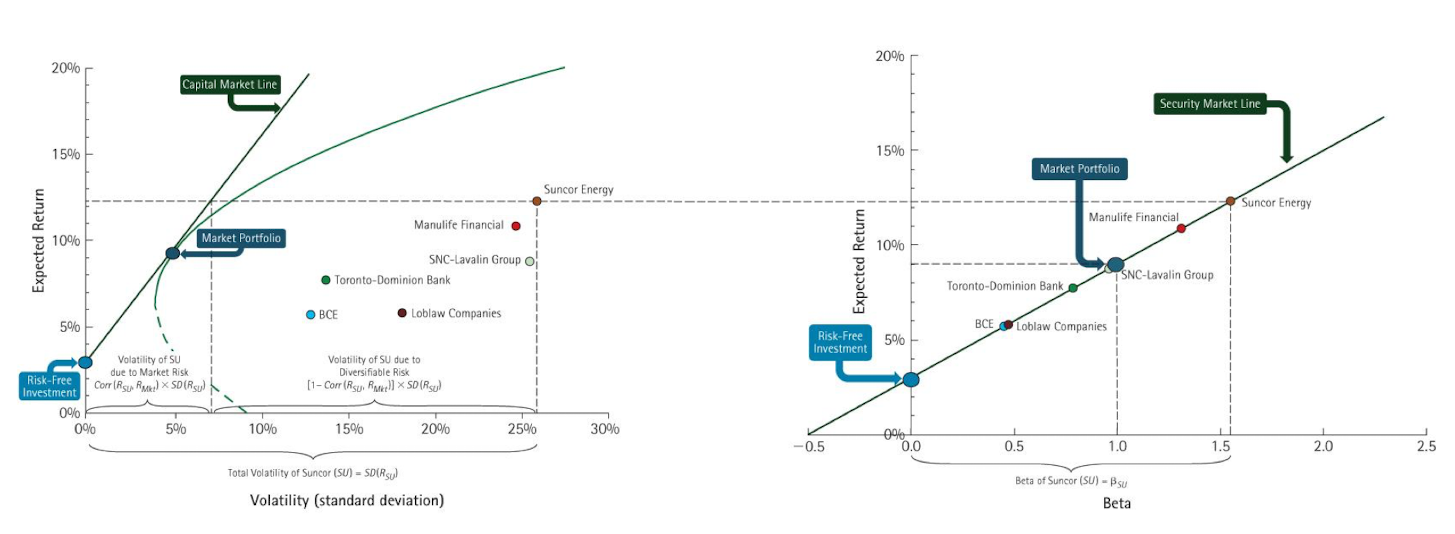
\includegraphics[scale=0.30]{Screenshot 2023-10-29 at 16.06.47.png}
\end{figure}

Notice that since the slope of the CML is the Sharpe ratio, the amount of volatility that is due to systematic risk is computed by 
\begin{equation*}
    \Corr(R_i, R_{\text{mkt}}) \times \Sd(R_i)
\end{equation*}
\subsubsection{Beta of a Portfolio}
The beta of a portfolio is the weighted average of the betas of the securities in the portfolio:
\begin{equation*}
    \beta_P = \sum_{i=1}^n x_i \beta_i
\end{equation*}

\section{CAPM and Cost of Capital}
\subsection{CAPM}
The CAPM allows us to identify the efficient portfolio of risky assets without having any knowledge of the expected return of each security. Recall that the CAPM is given by (\ref{capm}).
\subsubsection{Assumptions of CAPM}
\begin{enumerate}
    \item Investors can buy and sell all securities at competitive market prices (i.e.: no transaction costs) and can borrow/lend at the risk-free interest rate
    \item Investors hold only efficient portfolios of traded securities
    \item Investors have homogeneous expectations (everyone has same estimates of expected return, volatility, etc.)
\end{enumerate}
Given homogeneous expectations, all investors will demand the same efficient portfolio of risky securities - namely, the tangent portfolio, so the combined portfolio of risky securities of all investors must equal the tangent portfolio since this is the portfolio everyone invests in. Additionally, the sum of all investors' portfolios must equal the portfolio of all risky securities - namely the market portfolio. Thus, under the CAPM, the market portfolio equals the tangent portfolio.

\subsection{Empirical Estimation}
Note that the cost of capital of any investment equals the expected return of available investments with the same $\beta$, thus the CAPM provides an equation for the equity cost of capital.
\begin{definition}[Market index]
The market index reports the value of a particular portfolio of securities that make up the index.
\end{definition}
\begin{definition}[Price-Weighted Portfolio]
    A portfolio that holds an equal number of shares of each stock, independent of their size.
\end{definition}
\begin{definition}[Index funds]
    Mutual funds that invest in stocks in proportion to their representation in a published index.
\end{definition}
\begin{definition}[Exchange Traded Fund (ETF)]
    A security that trades directly on an exchange, like a stock, but represents ownership in a portfolio of stocks.
\end{definition}
\begin{definition}[Market proxy]
    A portfolio whose return closely tracks the true market portfolio.
\end{definition}
Consider when the price of a stock changes. This affects people's behaviour towards that stock, so do we continuously need to adjust the market portfolio when stock prices change? Define the total market value of a firm's outstanding shares to be 
\begin{equation*}
    MV_i = (\text{No. shares of $i$ outstanding}) \times (\text{Price of $i$ per share})
\end{equation*}
\begin{definition}[Value-Weighted Portfolio]
    A portfolio in which each security is held in proportion to its market capitalization. The weight of security $i$ in the portfolio is
    \begin{equation*}
        x_i = \frac{MV_i}{\sum_j MV_j}
    \end{equation*}
\end{definition}
By owning each stock in proportion to its market size, we own equal shares in each company, thus our ownership of each company is exactly the same. Additionally, if the prices of a stock change, then the weightings in the value-weighted portfolio will automatically shift \textbf{without trading}.

\subsubsection{Beta Estimation}
We can use linear regression to attempt to predict the return of a security:
\begin{equation*}
    (R_i - r_f) = \alpha_i + \beta_i(R_{\text{mkt}} - r_f) + \varepsilon_i 
\end{equation*}
where $\alpha_i$ is the intercept term and $\epsilon_i$ is the error term in estimation.
\begin{itemize}
    \item Under linear regression assumptions, $E[\varepsilon_i] = 0$
\end{itemize}
Under expectation, we have 
\begin{equation*}
    E(R_i) = r_f + \beta_i (E(R_\mkt - r_f) + \alpha_i
\end{equation*}
This shows us that $\alpha_i$ represents the distance above/below the SML. Since the SML is plotted by the CAPM, then when $\alpha_i = 0$, this means the security performed exactly as expected from the CAPM.
\begin{itemize}
    \item If $\alpha_i > 0$, the stock performed better than predicted by the CAPM
    \item If $\alpha_i < 0$, the stock performed worse than predicted by the CAPM
\end{itemize}

\subsection{Debt Beta}
Consider a bond with default probability $p$ and yield to maturity of $y$. If $L$ represents the expected loss per $\$1$ of debt in the event of default, then the expected rate of return of the bond is 
\begin{equation*}
    r_d = (1 - p)y + p(y - L) = y - pL
\end{equation*}
\begin{itemize}
    \item The average loss rate of unsecured debt is $60\%$
\end{itemize}
We can approximate debt betas using estimates of betas of bond indices by rating category. In general, debt betas tend to be low although they can be significantly higher for risky debt with a low credit rating and a long maturity.

\subsection{Arbitrage Pricing Theory}
A self-financing portfolio can be constructed by going long in some stocks and going short in others with equal market value. The Fama-French-Carhart Four Factor Specification gives the expected return of a stock relative to 4 different portfolios: 
\begin{enumerate}
    \item Market portfolio
    \item Small-minus-big portfolio - short selling a portfolio of big stock's returns
    \item High-minus-low portfolio - short selling stocks with a book-to-market ratio in at least the 70th percentile of stocks
    \item Prior one year momentum portfolio - After ranking stock returns from the previous year, long the top 30\% of stocks, which we finance by short selling the bottom 40\%
\end{enumerate}
\begin{equation*}
    E\left[R_s\right]=r_f+\beta_s^{M k t}\left(E\left[\mathrm{R}_{M k t}\right]-r_f\right)+\beta_s^{S M B} E\left[\mathrm{R}_{S M B}\right]+\beta_s^{H M L} E\left[\mathrm{R}_{H M L}\right]+\beta_s^{P R 1 Y R} E\left[\mathrm{R}_{P R 1 Y R}\right]
\end{equation*}

\section{Efficient Market Hypothesis}
\subsection{Investor Behaviour}
As described earlier, a stock's alpha is the difference between the stock's expected return and its required return according to the SML.
\begin{equation*}
    \alpha_s = E[R_s] - r_s
\end{equation*}
where 
\begin{equation*}
    r_s = r_f + \beta_s(E[R_\mkt] - r_f)
\end{equation*}
If we buy stocks where $E(R_s) > r_s$, aka when $\alpha_s > 0$, then the Sharpe ratio of a portfolio increases, so we can improve portfolio performance by buying stocks with $\alpha > 0$ (when market portfolio is inefficient). Similarly, we can also lower portfolio performance by buying stocks with $\alpha < 0$.
\begin{definition}[Rational expectations]
    All investors correctly interpret and use their own information
\end{definition}
\begin{itemize}
    \item If we assume everyone has rational expectations, then the market portfolio has an alpha of $0$ since the average of all portfolios is the market portfolio, thus the average alpha of all investors is $0$
    \item If no investor earns a negative, then none can earn a positive, so market portfolio is efficient
\end{itemize}
In the event that investors don't act on rational expectations or care about other aspects other than expected return and volatility, then the market portfolio is inefficient.
\begin{itemize}
    \item If individuals depart from the CAPM in random ways, the departures cancel out and the market portfolio is efficient
    \item If individuals systematically depart from the CAPM, then the departures won't cancel out and market prices/returns will be affected
\end{itemize}

\section{Financial Options}
\begin{definition}[Financal option]
    A contract that gives its owner the right (but not obligation) to purchase/sell an asset at a fixed price at some future date
    \item Price of an option depends on the price developments of the underlying asset
\end{definition}
There are 2 types of options:
\begin{enumerate}
    \item \textbf{Call option:} Gives the owner the right to \textit{buy} an asset
    \item \textbf{Put option:} Gives the owner the right to \textit{sell} an asset
\end{enumerate}
Basically, if you think the price of a stock will rise, you'd want to buy a call option. However, if you think the price will decrease, you'd want to buy a put option.
\begin{definition}[Strike Price]
    The price at which an option holder buys or sells a share of stock when the option is exercised
\end{definition}
\begin{definition}[Expiration Date]
    The last date on which an option holder has the right to exercise the option
\end{definition}
\begin{definition}[American Option]
    Options that allows holders to exercise the option on any date up to and including the expiration date
\end{definition}
\begin{definition}[European Option]
    Options that allow their holders to exercise the option only on the expiration date
\end{definition}
\begin{definition}[Option Premium]
    The market price of the option which compensates the seller for the risk of loss in the event that the option holder chooses the exercise the option
\end{definition}
\begin{definition}[In-the-money]
    Describes an option whose value if immediately exercised would be positive
\end{definition}
\begin{definition}[Out-the-money]
    Describes an option whose value if immediately exercised would be negative
\end{definition}

\subsection{Option Payouts at Expiration (Long)}
The value of owning a \textbf{call option} at expiration is 
\begin{equation*}
    C = \max(S - K, 0)
\end{equation*}
where $S$ is the stock price at expiration, $K$ the strike price.\\
The value of owning a \textbf{put option} at expiration is 
\begin{equation*}
    P = \max(K - S, 0)
\end{equation*}
The graphs of the option payouts at expiration are as follows:
\begin{figure}[h]
    \centering
    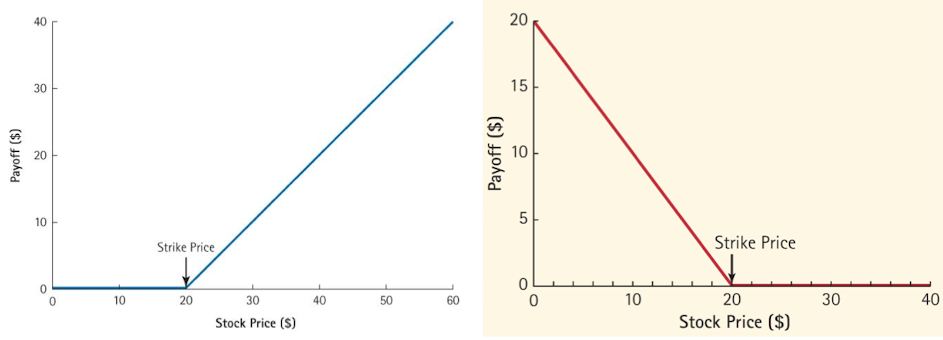
\includegraphics[scale=0.4]{Screenshot 2023-12-12 at 01.17.29.png}
\end{figure}

Its important to note that although \textit{payouts} of options in a long position are never negative, the \textit{profit} from purchasing and holding to expiration could be negative as the payout at expiration could be less than the ask price (the initial cost of the contract).

\subsubsection{Returns From Holding an Option to Expiration}
The maximum loss on a purchased call option is $100\%$, which is when the option expires worthless. This implies that $S - K < 0$, thus $C =0$. Since the buyer would allow the contract to expire rather than take a bigger loss from exercising the option, they lose 100\% of the money they put into buying the contract.\\
Similarly, the maximum loss on a purchased put option is 100\%, which is when the option expires worthless. This means $K - S < 0$, so $P = 0$. Usually, put options will have higher returns in states with low stock prices and are held generally not as an investment, but as a way to hedge other risk in a portfolio.

\subsection{Options Payouts at Expiration (Short)}
An investor selling an option contract holds a short position in the contract and has an obligation to sell/buy the option if the buyer chooses to exercise their contract.
\begin{figure}[h]
    \centering
    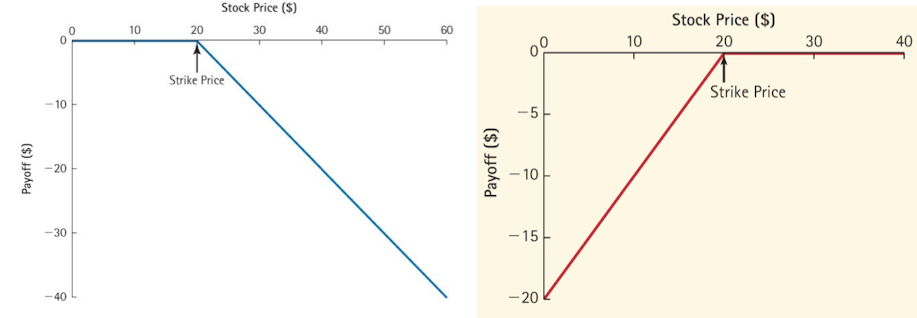
\includegraphics[scale=0.35]{Screenshot 2023-12-12 at 01.21.35.png}
\end{figure}

\subsection{Option Strategies}
\subsubsection{Straddle}
\begin{definition}
    A portfolio that holds a long position on a call option and put option at the same time on the same stock \textbf{with the same exercise date and strike price}
\end{definition}
\begin{itemize}
    \item Buy a straddle expecting a stock to be very volatile but unsure of which direction the stock will move in
\end{itemize}
\begin{figure}[h]
    \centering
    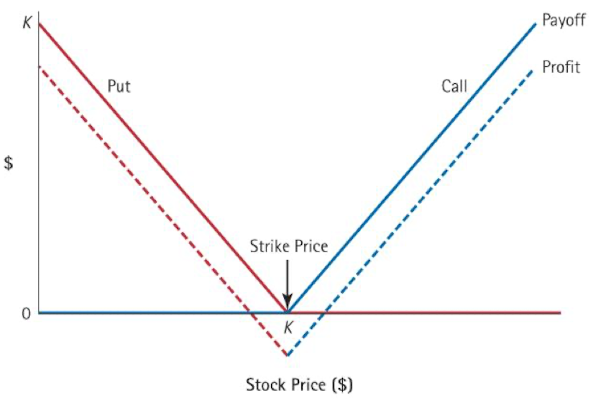
\includegraphics[scale=.25]{Screenshot 2023-12-12 at 01.35.22.png}
\end{figure}

\subsubsection{Strangle}
\begin{definition}
A portfolio that holds a long position in a call option and put option on the same stock with the \textbf{same exercise date but strike price on call exceeds strike price on put}
\begin{itemize}
    \item Buy a strangle when feel that a positive movement is more likely but want to have some insurance against downward swings
\end{itemize}
\end{definition}
\begin{figure}[h]
    \centering
    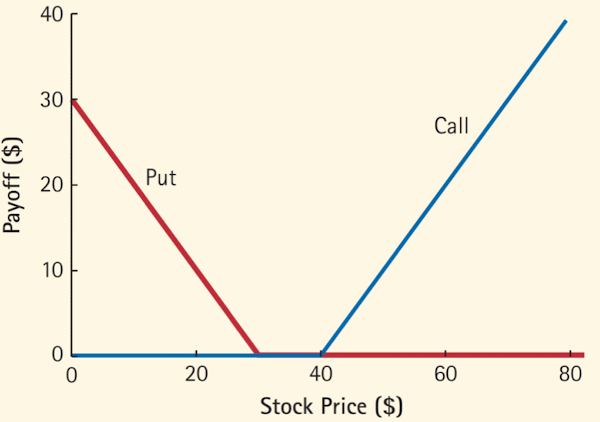
\includegraphics[scale=0.20]{Screenshot 2023-12-12 at 01.44.08.png}
\end{figure}

\subsubsection{Butterfly Spread}
\begin{definition}
    Long two call options at differing strike prices, short two call options at a strike price equal to the average strike prices of the two long options
    \begin{itemize}
        \item Makes money when stock and strike prices are close (opposite to straddle), buy when not expecting much volatility
    \end{itemize}
\end{definition}
\begin{figure}[h]
    \centering
    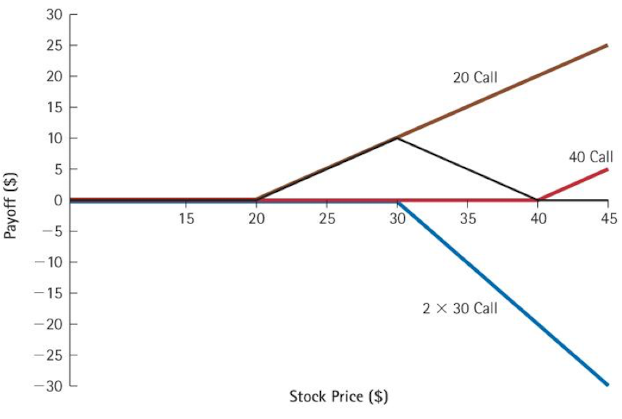
\includegraphics[scale=0.25]{Screenshot 2023-12-12 at 01.46.48.png}
\end{figure}

\subsubsection{Covered Call}
A covered call is when you purchase a stock and write a call against it. The call writer gives up any stock value above $K$ in return for the initial premium, so if you planned to sell stock above price $K$ anyways, the call imposes a sort of ``sell discipline", hence investors use this strategy when not expecting large price increases. 
\begin{center}
\begin{tabular}{ccc} 
& $\mathbf{S}_{\mathrm{T}} \leq \mathbf{K}$ & $\mathbf{S}_{\mathrm{T}}>\mathbf{K}$ \\
\hline Payoff of stock & $\mathbf{S}_{\mathrm{T}}$ & $\mathbf{S}_{\mathrm{T}}$ \\
+ Payoff of written call option & $\mathbf{0}$ & $-\left(\mathbf{S}_{\mathrm{T}}-\mathbf{K}\right)$ \\
\hline = Total & $\mathbf{S}_{\mathrm{T}}$ & $\mathbf{K}$
\end{tabular}
\end{center}

\subsection{Put-Call Parity}
A protective put is when an investor purchases a stock and buys a put option to act as a sort of insurance against downside. 
\begin{center}
\begin{tabular}{ccc} 
& $\mathbf{S}_{\mathrm{T}} \leq \mathbf{K}$ & $\mathbf{S}_{\mathrm{T}}>\mathbf{K}$ \\
\hline 
Payoff of stock & $\mathbf{S}_{\mathrm{T}}$ & $\mathbf{S}_{\mathrm{T}}$ \\
+ Payoff of bought put option & $\mathbf{K}-\mathbf{S}_{\mathrm{T}}$ & $\mathbf{0}$ \\
\hline
= Total & $\mathbf{K}$ & $\mathbf{S}_{\mathrm{T}}$
\end{tabular}
\end{center}
Another strategy is to purchase a bond that pays $K$ in one year and buying a call option.
\begin{center}
\begin{tabular}{ccc} 
& $\mathbf{S}_{\mathrm{T}} \leq \mathbf{K}$ & $\mathbf{S}_{\mathrm{T}}>\mathbf{K}$ \\
\hline 
Payoff of bond & $\mathbf{K}$ & $\mathbf{K}$ \\
+ Payoff of bought call option & $\mathbf{0}$ & $\mathbf{S}_{\mathrm{T}}-\mathbf{K}$ \\
\hline
= Total & $\mathbf{K}$ & $\mathbf{S}_{\mathrm{T}}$
\end{tabular}
\end{center}
Notice how the payoffs of both strategies are the same. By the Law of One Price, they must have the same price, so 
\begin{equation*}
    S + P  = PV(K) + C
\end{equation*}
Rearranging, we get 
\begin{equation*}
    C = S + P - PV(K)
\end{equation*}
which is the price of a European call option with a non-dividend paying stock. If the stock does pay dividends, then 
\begin{equation*}
    C = S + P - PV(K) - PV(\text{Div})
\end{equation*}
This relationship is known as the \textbf{put-call parity}.

\subsection{Factors Affecting Option Prices}
\begin{itemize}
    \item An American option can't be worth less than its European counterpart
    \begin{itemize}
        \item Or else there's no incentive to hold to expiration
    \end{itemize}
    \item A put option can't be worth more than its strike price
    \begin{itemize}
        \item Or else $\max(K-S, 0) > K \implies K < 0$ or $S < 0$
    \end{itemize}
    \item A call option can't be worth less than the stock itself
    \begin{itemize}
        \item Or else $\max(S-K, 0) > S \implies K < 0$ or $S < 0$
    \end{itemize}
\end{itemize}
\begin{definition}[Intrinsic value]
    The amount by which an option is in-the-money, or zero if out-the-money
\end{definition}
\begin{itemize}
    \item An American option can't be worth less than its intrinsic value, or else everyone will fulfill instantly since value of the option will be worth more instantly 
\end{itemize}
\begin{definition}[Time Value]
    The difference between an option's price and its intrinsic value
\end{definition}
\begin{itemize}
    \item An American option can't have a negative time value, or else its intrinsic value is less than its price, AKA its worth more than is intrinsic value
\end{itemize}


\subsection{Option Valuation}






\end{document}
